% Linear script scrub: project hidden states onto nullspace of learned subspace
\documentclass[tikz,border=5pt]{standalone}
\usepackage{xcolor}
\usepackage{fontspec}
\usetikzlibrary{arrows.meta,shapes.geometric,shadows.blur,positioning}

% Define color scheme
\definecolor{primaryblue}{RGB}{41,128,185}
\definecolor{secondarygreen}{RGB}{39,174,96}
\definecolor{accentorange}{RGB}{230,126,34}
\definecolor{warningred}{RGB}{231,76,60}
\definecolor{lightgray}{RGB}{236,240,241}
\definecolor{darkgray}{RGB}{52,73,94}

\begin{document}
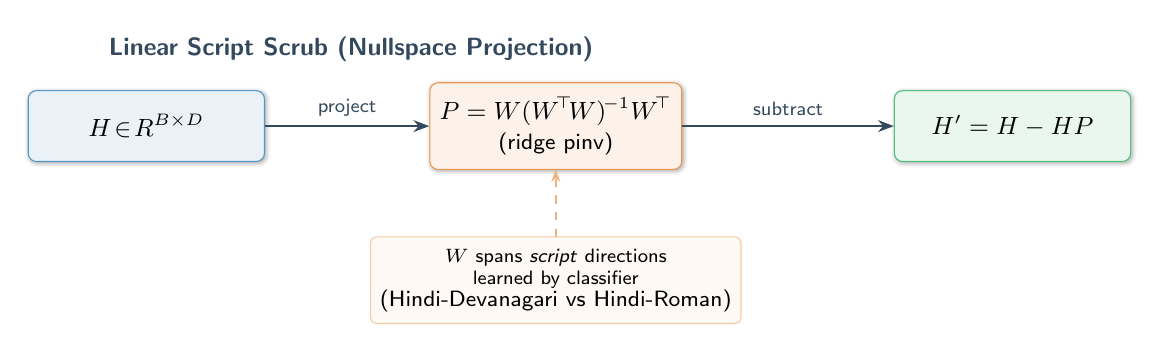
\begin{tikzpicture}[
  node distance=12mm and 18mm,
  block/.style={
    draw=primaryblue!80,
    fill=primaryblue!10,
    rounded corners=3pt,
    minimum width=30mm,
    minimum height=9mm,
    align=center,
    font=\sffamily\small,
    blur shadow={shadow blur steps=5, shadow xshift=0.5pt, shadow yshift=-0.5pt}
  },
  projblock/.style={
    draw=accentorange!80,
    fill=accentorange!10,
    rounded corners=3pt,
    minimum width=32mm,
    minimum height=11mm,
    align=center,
    font=\sffamily\small,
    blur shadow={shadow blur steps=5, shadow xshift=0.5pt, shadow yshift=-0.5pt}
  },
  resultblock/.style={
    draw=secondarygreen!80,
    fill=secondarygreen!10,
    rounded corners=3pt,
    minimum width=30mm,
    minimum height=9mm,
    align=center,
    font=\sffamily\small,
    blur shadow={shadow blur steps=5, shadow xshift=0.5pt, shadow yshift=-0.5pt}
  },
  line/.style={-{Stealth[length=2mm]}, thick, draw=darkgray}
]

% Input hidden states
\node[block] (hin) at (0,0) {$H \!\in\! \mathbb{R}^{B\times D}$};

% Projection matrix
\node[projblock] (proj) at (52mm,0) {$P = W (W^{\!\top}\!W)^{\!-1} W^{\!\top}$\\{\footnotesize (ridge pinv)}};

% Output scrubbed states
\node[resultblock] (hout) at (110mm,0) {$H' = H - H P$};

% Main flow arrows
\draw[line] (hin) -- (proj) node[midway, above, font=\sffamily\scriptsize, text=darkgray] {project};
\draw[line] (proj) -- (hout) node[midway, above, font=\sffamily\scriptsize, text=darkgray] {subtract};

% Annotation box below
\node[align=center, draw=accentorange!40, fill=accentorange!5, rounded corners=2pt,
      minimum width=32mm, minimum height=11mm, font=\sffamily\scriptsize]
  at ($(proj.south)+(0,-14mm)$)
  {$W$ spans \textit{script} directions\\learned by classifier\\{\footnotesize (Hindi-Devanagari vs Hindi-Roman)}};

% Connect annotation to projection block
\draw[-{Stealth[length=1.5mm]}, dashed, thick, draw=accentorange!60]
  ($(proj.south)+(0,-14mm)+(0,5.5mm)$) -- (proj.south);

% Add title
\node[anchor=north, font=\sffamily\bfseries\small, text=darkgray]
  at ($(hin.north)+(26mm,8mm)$) {Linear Script Scrub (Nullspace Projection)};

\end{tikzpicture}
\end{document}
